#let beaglebone-nunchuk = false
#let beaglebone-nunchuk = false
#if training == "yocto" {#let beaglebone-nunchuk = true}
#if training == "buildroot" {#let beaglebone-nunchuk = true}
#if training == "embedded-linux" {#let beaglebone-nunchuk = true}
#if training == "linux-kernel" {#let beaglebone-nunchuk = true}

#let beaglebone-audio = false
#let beaglebone-audio = false
#if training == "embedded-linux" {#let beaglebone-audio = true}

#import "@local/bootlin:0.1.0": *

#import "@local/bootlin-yocto:0.1.0": *

#import "@local/bootlin-utils:0.1.0": *

#import "../../typst/local/themeBootlin.typ": *

#import "../../typst/local/common.typ": *

#show: bootlin-theme.with( aspect-ratio: "16-9", config-common(handout: "handout" in sys.inputs and sys.inputs.handout == "1", ))

#show raw.where(block: true): set block(fill: luma(240), inset: 1em, radius: 0.5em, width: 100\%)

#show raw.where(block: true): set text(size: 11pt)

#show raw.where(block: false): r => text(fill: color-link)[#r]

#show raw.where(lang: "c", block: true): set block(fill: luma(240), inset: 0.4em, radius: 0.5em, width: 95\%, breakable: true, above: 12pt, below: 12pt)

#show raw.where(lang: "c", block: true): set text(11pt)

#show raw.where(lang: "console", block: true):set block(fill: luma(240), inset: 0.4em, radius: 0.5em, width: 95\%, breakable: true, above: 6pt)

#show raw.where(lang:"console", block: true): set text(12pt)

=== Beaglebone Black / Beaglebone black wireless shopping list
  \begin{columns}
    #table(columns: (50\%, 50\%), stroke: none,\n[
    \footnotesize
    \begin{itemize}
      \item BeagleBone Black or BeagleBone Black Wireless, from
            \href{https://beagleboard.org}{BeagleBoard.org}
            \begin{itemize}
                \item Texas Instruments AM335x (ARM Cortex-A8 CPU)
                \item 512 MB of RAM
                \item 4 GB of on-board eMMC storage
                \item Plenty of peripherals and features
                \item 2 x 46 pins headers, with access to many expansion buses
                (I2C, SPI, UART and more)
            \end{itemize}
    \item MicroUSB cable
    \item USB Serial Cable - 3.3 V - Female ends (for serial console)
      \footnote{\tiny \url{https://www.olimex.com/Products/USB-Modules/Interfaces/USB-SERIAL-F}}
    
#if beaglebone-nunchuk {
    \item Nintendo Nunchuk with UEXT connector
      \footnote{\tiny \url{https://www.olimex.com/Products/Modules/Sensors/MOD-WII/MOD-Wii-UEXT-NUNCHUCK/}}
    \item Breadboard jumper wires - Male ends (to connect the Nunchuk)
      \footnote{\tiny \url{https://www.olimex.com/Products/Breadboarding/JUMPER-WIRES/JW-110x10/}}
    }{}
    \item MicroSD card
    
#if beaglebone-audio {
    \item A standard USB audio headset
    }{}
    \end{itemize}
    ],[
    \begin{center}
      \includegraphics[width=0.6\textwidth]{slides/shopping-list-beaglebone/beagleboneblack.png}\\
      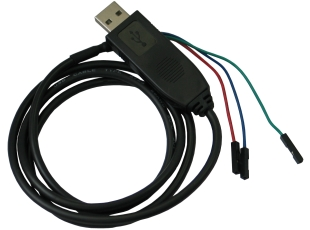
\includegraphics[width=0.6\textwidth]{common/usb-serial-cable-female.png}\\
      
#if beaglebone-nunchuk {
      \includegraphics[width=0.6\textwidth]{common/nunchuk.jpg}\\
      \includegraphics[width=0.6\textwidth]{common/jumper-wires.jpg}\\
      }{}
      
#if beaglebone-audio {
      \includegraphics[width=0.6\textwidth]{common/usb-audio.png}\\
      }{}
    \end{center}
  \end{columns}
  ])

